\section{Aufbau}
\label{sec:Aufbau}

Der Aufbau ist schematisch in Abbildung~\ref{fig:aufbau} zusehen.
Als Quelle der $γ$-Strahlung wird für alle Messungen ${}^{137}$Cs verwendet.
Vor die Quelle wird ein Bleiabsorber mit einem
Loch mit $\SI{3}{\milli\meter}$ Durchmesser gestellt, welcher den Strahl kollimiert.
Dahinter wird eine drehbare Plattform für die Würfel eingebaut,
auf den innerne Aufbau der Würfel wird in Kapitel~\ref{sec:durchfuehrung} eingegangen.
Dahinter befindet sich der Natriumiodid Szintillationsdetektor.
Das Ausgangssignal wird in einem Multichannelanalyzer in Bins aufgeteilt.
Ein Bin entspricht dabei einem Energieintervall.
Diese können am Computer dargestellt und ausgewertet werden.

\begin{figure}
  \centering
  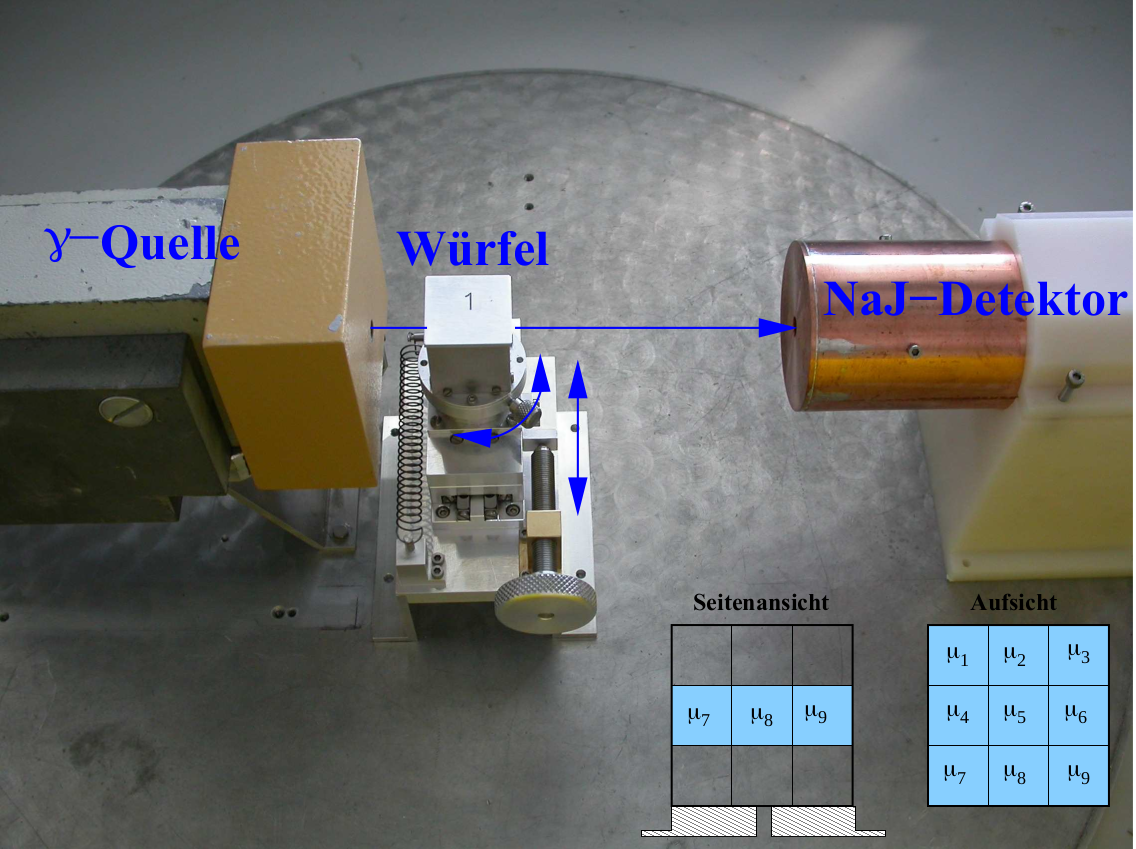
\includegraphics[width=0.8\textwidth]{pdfs/aufbau_v14.png}
  \caption{Versuchsaufbau aus der Anleitung. \cite{anleitung}}
  \label{fig:aufbau}
\end{figure}

\section{Durchführung}
\label{sec:durchfuehrung}
Zuerst wird das Spektrum der Cs-Quelle aufgenommen. Dazu werden über einen
Messzeitraum von $\SI{100}{\second}$ die Häufigkeitsverteilung der Bineinträge aufgenommen, welcher
ein Multichannelanalyzer liefert.

Es sind vier Würfel gegeben. Nr. 1 besteht nur aus einem Aluminiumgehäuse
und ist ansonsten hohl. Würfel Nr. 2 und Nr. 3 haben auch ein
Aluminiumgehäuse doch die 27 inneren Würfel bestehen aus einem unbekannten
Material. Würfel Nr. 5 besteht aus einer Mischung aus Material 2 und 3 der
markierten Würfel.
Von den Würfeln wird in Seitenansicht, Abbildung~\ref{fig:aufbau},
nur die mittlere Ebene an kleineren Würfeln vermessen.
Die Bezeichung der Würfel ist gleich mit der in Abbildung~\ref{fig:projection}.
Angefangen wird damit, ein Spektrum aufzunehmen, während Würfel 1 im
Strahlengang steht. Dieser Vorgang wird für alle 12, oben angegebenen,
Richtungen durchgeführt.
Diese Messung wird später benötigt, um den Einfluß des Gehäuses zu
beurteilen.
Die Messzeit wird mit $\SI{60}{\second}$ gewählt.

Danach wird analog für Würfel 2 und 3 verfahren, mit der Änderung,
dass nur vier der 12 Richtungen durch den jeweiligen Würfel benötigt werden.
Die Anzahl an Messungen kann verringert werden, da der Würfel homogen ist.
Die Messzeiten betragen $T_2 = \SI{150}{\second}$ und $T_3 = \SI{100}{\second}$.

Zuletzt wird Würfel~5, wie Würfel~1, bei einer Messzeit von
$\SI{100}{\second}$ pro Richtung vermessen.
